\documentclass{standalone}
\usepackage{tikz}
\usetikzlibrary{graphs,quotes,positioning}

\begin{document}

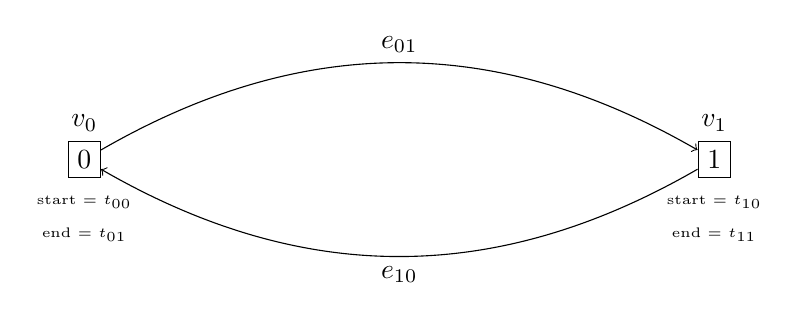
\begin{tikzpicture}
    \graph [nodes = {rectangle, draw},
                    circular placement,
                    radius = 2cm] {
                        0[xshift=-3cm, label=$v_0$] ->[bend left, "$e_{01}$"] 1[yshift=-1cm, xshift=5cm, label=$v_1$],
                        1 ->[bend left, "$e_{10}$"] 0
                        };
                        \node[below=0.1cm of 0] (n1) {\tiny start = $t_{00}$};
                        \node[below=0.0001cm of n1] (n2) {\tiny end = $t_{01}$};

                        \node[below=0.1cm of 1] (n3) {\tiny start = $t_{10}$};
                        \node[below=0.0001cm of n3] (n4) {\tiny end = $t_{11}$};
\end{tikzpicture}
\end{document}